\section*{Quality Control of raw reads}

We used LongQC and FASTQC to calculate basic technical statistics and evaluate the quality of \ac{HiFi} raw reads~\cite{fukasawaLongQCQualityControl2020,BabrahamBioinformaticsFastQC}. The length of the 1,747,253 raw reads follows a unimodal distribution with an average size of 13.5 kb. The longest read is 46.7 kb long. \\

The quality reports show no issues except for the GC distribution, which exhibited a bimodal distribution. Instead of the expected normal distribution, we observed two peaks, around 45\%  and 37\%, respectively. We trimmed 25 sequences at 3' and 5' using LongQC. Despite the minimal impact of these, we used the trimmed sequences for the remainder of the analysis. \\

\section*{Modeling reads of T. vulgaris to T. quinquecostatus reference genome}

Although not included in this report, we experimented with different subset sizes, alignment tools, and window sizes. These experiments produced consistent results. Regarding the number of iterations and chains, various experiments with both experimental and simulated data justified a conservative choice, as we obtained equivalent results in all cases using fewer computational resources. \\

The posterior sampling distribution obtained using Bayesian inference for each chromosome independently is shown in \autoref{fig:bayesian_posterior}. Notice that we are using the number of mapped reads per window and not the number of mapped nucleotides. We made this decision to reduce the computational cost. \\

\graphicspath{{gfx/}}
\begin{sidewaysfigure}
\begin{center}
    \input{gfx/05-posterior_var_edited.pdf_tex}
    \caption{Posterior sampling distribution of mapped reads according a Zero-inflated Poisson process}    
    \label{fig:bayesian_posterior}    
\end{center}
\footnotesize
The posterior sampling distributions were obtained by modeling the number of mapped reads per 1000-length windows according to the model specified by \eqref{eq:model} using \ac{MCMC}.   
\end{sidewaysfigure}    

\section*{De novo assembly of T. vulgaris and homology-based assembly scaffolding}

As discussed in \autoref{cha:Methods}, we obtained a \textit{de novo} assembly from our \ac{HiFi} long reads, hereafter draft assembly, and a scaffolded assembly using RagTag. We did the scaffolding process according to a whole-genome alignment sequence with Minimap2. As an example, we show in \autoref{fig:sinteny} how four contigs were oriented and arranged. The covered regions of the \textit{T. quinquecostatus} genome are shown in \autoref{fig:coverage_long_reads}. The whole-genome alignment covers most of the "telomeric" regions for the 13 pseudo-chromosomes but presents large uncovered areas, especially near the middle of the pseudo-chromosome. In total, 47.3\% of the \textit{T. quinquecostatus} genome is uncovered. \\

\begin{figure}
\begin{center}
    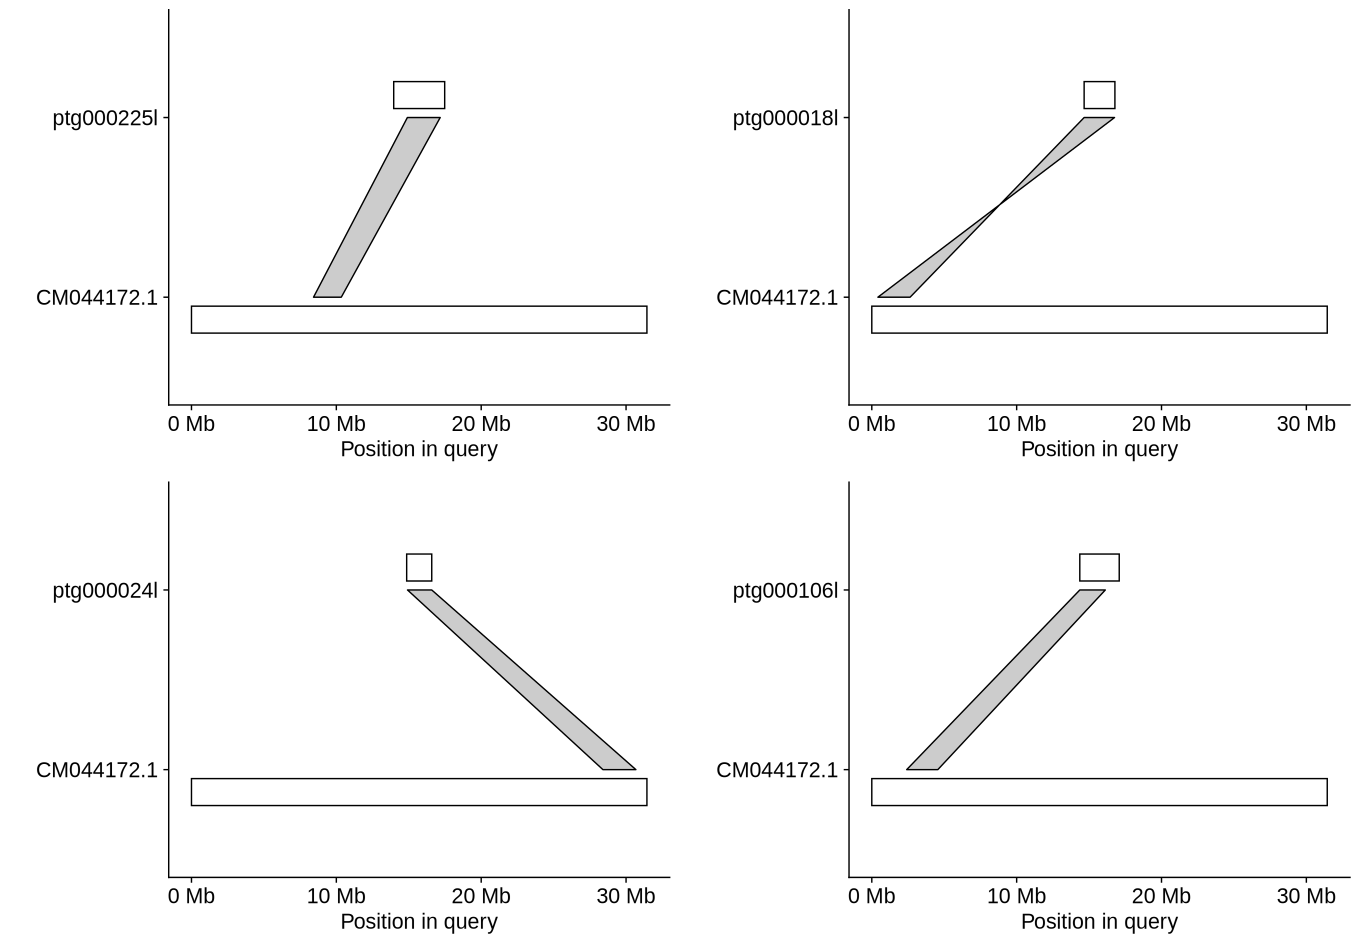
\includegraphics[width=\textwidth]{gfx/CM044172.1_sinteny.pdf}
    \caption{Sinteny-like plot of pseudochromosome CM044172.1}  
    \label{fig:sinteny}    
\end{center}
\footnotesize
We show the alignments of the largest four \textit{de novo} contigs of \textit{T. vulgaris} mapped to \textit{T. quinquecostatus}. This visualization corresponds to how we arrange and orient the contigs in the scaffolding process. 
\end{figure} 

\begin{figure}
    \begin{center}
        \includegraphics[width=\textwidth]{gfx/coverage_long_reads_tq.pdf}
        \caption{Coverage of \textit{T. vulgaris} and \textit{T. quinquecostatus} whole-genome alignment}   
        \label{fig:coverage_long_reads}
 
    \end{center}
        \footnotesize
    We show the spatial distributions of the \textit{de novo} \textit{T. vulgaris} contigs when aligning those to the reference genome of   \textit{T. quinquecostatus}. We include only the primary alignment whose length is greater than 1000, as those are the ones RagTag will use for the scaffolding process. We represent the alignments only to the 13 pseudo-chromosomes.  
\end{figure}   

We calculated the gap sizes according to \eqref{eq:infergapsize}. However, 91.7\% of the inferred gaps have an unknown size rather than an inferred one, as in most cases, the inferred size was greater than the threshold established. By convention, gaps of unknown size have a  length of 100 bp, indicating that we do not have enough information to establish the gap size.\cite{AGPSpecificationV2}\\

The scaffolding process placed 880 contigs (77\% of base pairs) into bigger supercontigs.  Interestingly, a few of the contigs of the draft assembly aligned not to the \textit{T. quinquecostatus} pseudo-chromosomes but to its unplaced contigs. We generated 13 supercontigs by joining the adjacent contigs of the draft assembly that aligned to each of the 13 pseudo-chromosomes of \textit{T. quinquecostatus} (supported by \ac{Hi-C} experimental data). Therefore,  these supercontigs are a reconstruction of the \textit{T. vulgaris} pseudo-chromosomes based on the pseudochromosome similarity of \textit{T. quinquecostatus} and \textit{T. vulgaris}.\\

\section*{Assembly quality assessment}

We show global statistics comparing the draft and the scaffolded assembly in \autoref{tab:global}, calculated with assembly-stats. Regarding BUSCO results, the assembly achieved a completeness score of 96.4\%, with 65.0\% and 31.4\% of the genes classified as "complete and single copy" and "complete and duplicated," respectively. The false positive rate is 0.6\%, and the misclassification rate is 3.0\%. The analysis was performed on 2326 BUSCO genes. 

\begin{table}[h!]
    \begin{minipage}{\linewidth}
    \renewcommand\thefootnote{\thempfootnote}
    \centering
    \begin{tabular}{@{}cccccc@{}}
        \toprule
        Metric              & N\footnote{Number of scaffolds}    & Ave (Mb)\footnote{Average length of the scaffolds} & Largest (Mb)\footnote{Largest scaffold} & N50 (Mb)\footnote{Length such that scaffolds of this length or longer include half the bases of the assembly. The number of scaffold, $n$ is also included.}     & Ns\footnote{Number of Ns ambiguous nucleotides}      \\ \midrule
        Draft assembly      & 1,884 & 0.48     & 11.17        & 1.87 ($n$=133) & 0       \\
        Scaffolded assembly & 1,065 & 0.86     & 95.24        & 48.92 ($n$=8)  & 2,536,928 \\ \bottomrule
        \end{tabular}
        \caption{Comparison of global statistics between the draft and scaffolded assembly}
        \label{tab:global}
\end{minipage}
\end{table}

According to cytometric estimations, the \textit{T. vulgaris} haploid genome size is 754.60 Mb (1C\footnote{The amount of DNA contained within a haploid nucleus} = 0.77pg).~\cite{marieCytometricExercisePlant1993,PlantDNACvalues} The size of our 13 pseudo-chromosomes is 695.63 Mb. In addition, if we consider the sum of the 48 super contigs placed by homology with unplaced \textit{T. quinquecostatus} contigs, the number is closer to the estimation:  706.41Mb. However, the size of the whole assembly exceeds the estimate; 911.87Mb.\\


\section*{Mapping short Illumina reads to scaffolded assembly}

\autoref{fig:error_rate} shows the result of mapping the Illumina reads of the five individuals to the scaffolded assembly. The two \textit{S. montana} individuals are grouped in the plot, showing similar mapping patterns to the scaffolded assembly of \textit{T. vulgaris}. They have a lower percentage of properly mapped sequences than the other \textit{T. vulgaris} specimens. The use of hybridization two, the more stringent procedure, increases the percentage of mapped reads and the number of mismatches in both \textit{S. montana} individuals.\\

Although the increased number of mapped reads also affects \textit{T. vulgaris} individuals, it is less pronounced. The use of hybridization two does not increase the number of mismatches in \textit{T. vulgaris} as it does in \textit{S. montana}. The differences in the percentage of mapped reads between \textit{T. vulgaris} individuals are slight, but the individual Thym607 used to construct the assembly has the lowest number of mismatches. Although we achieved better mapping results by penalizing \ac{SNP}s and indels (insertions or deletions) more than the default parameters, we used default parameters for a more appropriate comparison.\\



\begin{figure}
    \begin{center}
        \def\svgwidth{\textwidth}
        \input{gfx/mapped_vs_error_rate.pdf_tex}
        \caption{Results of aligning Illumina short reads to the assembly under two hybridization conditions}            
        \label{fig:error_rate}
    \end{center}
    \footnotesize
    We show the percentage of properly paired reads (with consistent orientation and distance within forward and reverse read) and the percentage of mismatches of the Illumina short reads of 5 different individuals (see \autoref{tab:illumina_samples}). Each specimen was sequenced using two different hybridization protocols for the scaffolded assembly.     
\end{figure}   

Since these reads have been sequenced using baits technology, the coverage cannot be used as a validation of our reference genome. Using hybridization condition one, 74.61\% of the reference genome is uncovered. Using hybridization condition two, this number is even higher: 92.50\%. 